\section{Event Selection}
\subsection{Search Strategy}
\label{sect:cuts}
In this analysis, two leptons are created with two missing particles, so \mttwo can be a good descriminator to separate signal 
from the SM backgrounds that leptons are produced from W or Z boson. When the mass difference between the chargino and neutralino 
is suffuciently large, \mttwo can exceed 80 GeV which is the maxmimum of the \mt of a lepton which comes from the decay of a W boson.
When the mass difference is not sufficiently large, \mttwo of the signal events is below 80 GeV and the signal is buried under the W+jets
backgrounds. In such conditions, $\Sigma\,\mt$ which is defined as $\mt_{,\ell1} + \mt_{,\ell2}$ can be useful to distinguish between the signal and 
SM backgrounds.
To optimize the cuts, two signal points are selected, one with a high mass difference ($m_{\chipm}$ = 380\,\GeV and $m_{\chiz}$ = 1\,\GeV) and
another one with a low mass difference ($m_{\chipm}$ = 180 GeV and $m_{\chiz}$ = 60 GeV). An optimized cut should minimize the signal strength, 
which is the ratio of the measured upper limit on the cross section and the theoretical signal cross section. The details of the statistical 
method can be found in section \ref{sect:stat}.

\subsection{\texorpdfstring{$\tauTau$ Channel}{tau-tau Channel}}
\label{sect:tauTauCuts}
%In the context of MSSM, supersymmetric objects are produced in pairs to conserve R-parity quantum number. Therefore in the production of charginos from proton-proton collisions, one may consider the following interaction $$pp\rightarrow\PSGcpDo\PSGcmDo\rightarrow\sTau^{+}\nu_\tau \sTau^{-}\nu_\tau\rightarrow\tau^{+}\PSGczDo\nu_\tau\tau^{-}\PSGczDo\nu_\tau\rightarrow\tau^{+}\tau^{-} + 2\,\PSGczDo + 2\,\nu_\tau.$$ In the detector, what can be observed are only 2 tau leptons plus missing transverse energy from the presence of neturinos and neutralinos in the final state.\\
%The tau leptons can decay leptonically, in 35\% of the time, or can decay via hadrons, which is occuring with 65\% of probability. Since there are two leptons in the final state, then the probability of having $\PSGcpDo\PSGcmDo \rightarrow \hadtau+e/\mu+\MET$ is about 46\%, while the probability of occuring $\PSGcpDo\PSGcmDo \rightarrow \hadtau+\hadtau+\MET$ is about 42\%. Hereafter, final states containing a lepton are referred to as $\leptonTau$ channel and those events where the two taus decays via hadrons are referred to as $\tauTau$. This section describes the cuts to enhance $\tauTau$ events. The list of cuts to select the $\leptonTau$ events can be found in Section~\ref{sect:leptonTauCuts}.\\    
In the final state with 2 hadronic taus, events are required to pass the following list of cuts
\begin{itemize}
\item at least two reconstructed opposit-sign tau objects, with $\pt>45\GeV$ and $|\eta|<2.1$, are required;\\ Since the online trigger cuts require two taus with $\pt>35\GeV$, then it can be justified to have an offline cut on $\pt>45\GeV$. 
\item both taus are required to pass medium isolation criteria;\\ In the online selection, it is also required two medium isolated taus.
\item extra muons and leptons are vetoed;\\ In order to reject background from di-boson events, events with extra leptons are failed for further analysis.
\item the invariant mass of the two taus, $m_{\tau\tau}$, should be above 12 \GeV;\\ This cut removes backgrounds from multi-jet events. 
\item events under the Z mass peak are rejected, namely $|m_{\tau\tau}-m_{\Z}^{\rm rec}|>15\GeV$;\\ This requirement acts against DY background events. 
\item A cut on $\mindphifour$ is applied to be above 1;\\ This cut is introduced against multi-jet events.   
\item $\mttwo>40\GeV$. 
\end{itemize}
After applying pre-selection cuts, two extra set of cuts are introduced, where each of them is sensitive to some regions of $\chione\PSGczDo$ mass plane: one aimed the regions with large mass difference between charginos and neutralinos, the other one is dedicated for low mass regions. It should be noted that the two search bins are chosen to be exclusive in order to be able to combine the statistics at the end.
A first set of cuts includes a cut on $\mttwo$.
\begin{itemize}
\item $\mttwo>90\GeV$.
\end{itemize}
A second set of cuts includes some cuts on different variables listed below.
\begin{itemize}
\item $\mttwo<90\GeV$;
\item $\SumMT>250\GeV$;
\item b-jets tagged with CSVM algorithm are vetoed.
\end{itemize}
Two cut flow tables according to each of search bins are presented, which can be found in Tables~\ref{tbl:cutflowtable1} and~\ref{tbl:cutflowtable2}. The SUSY signal points used in the tables and figures correspond to $(m_{\chione}=240\GeV,m_{\PSGczDo}=40\GeV)$.   
%\begin{sidewaystable}
\begin{table}
\begin{center}
\begin{tabular}{lcccccccc}
\hline\hline
  &SUSY&QCD&VV&W ($\ell\nu$)&DY&Top&Total Bkg&\\
\hline\hline
pre-selection &10.90&135.29&1.11&31.93&13.17&5.26&186.76$\pm$135.47&\\
$\mttwo>90\GeV$&4.10&0.00&0.02&0.00&0.56&0.00&0.58$\pm$0.07&\\
\hline\hline
\end{tabular}
\caption{Cut-flow-table for $\tauTau$ channel: search bin\#1.}
\label{tbl:cutflowtable1}
\begin{tabular}{lcccccccc}
\hline\hline
  &SUSY&QCD&VV&W ($\ell\nu$)&DY&Top&Total Bkg&\\
\hline\hline
pre-selection &10.90&135.29&1.11&31.93&13.17&5.26&186.76$\pm$135.47&\\
$\mttwo < $ 90 &6.80&135.29&1.09&31.93&12.60&5.26&186.17$\pm$135.47&\\
$\SumMT > $ 250 &3.85&0.00&0.23&1.02&0.83&2.63&4.71$\pm$1.49&\\
b-jet veto &3.13&0.00&0.15&0.43&0.81&0.53&1.91$\pm$0.87&\\
\hline\hline
\end{tabular}
\caption{Cut-flow-table for $\tauTau$ channel: search bin\#2.}
\label{tbl:cutflowtable2}
\end{center}
\end{table}
%\end{sidewaystable}
The distributions of $\mttwo$ and $\SumMT$ after applying pre-selection cuts are shown in Figure~\ref{fig:comparison}. There is only one QCD event with slightly large weight contributing to the plots. Hence the disagreement between data and MC in a couple of bins of $\SumMT$ distribution can be justifed. In order to be blind to data, in both distributions data events are not shown at some points. Overally, it can be concluded that data and MC are in reasonable agreement. 
\begin{figure}[htbp]
\centering
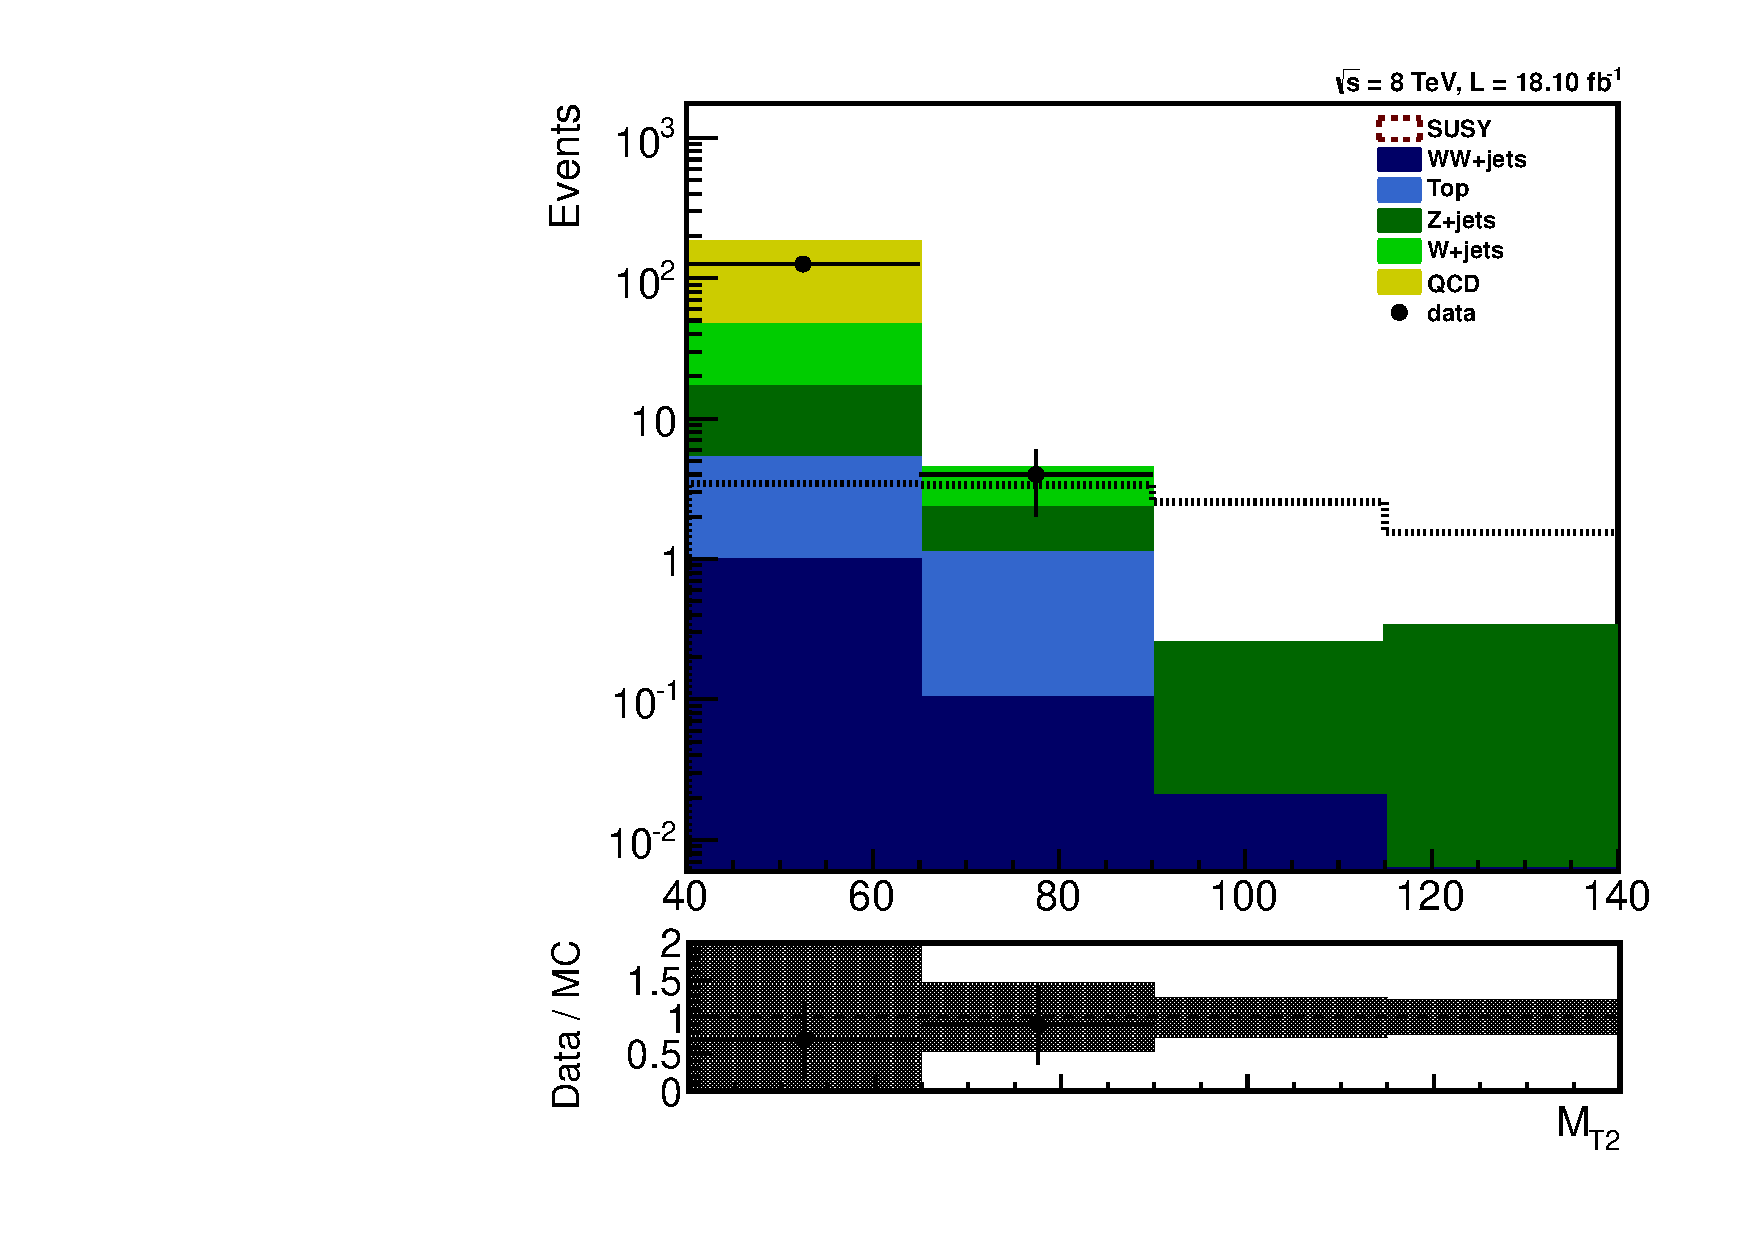
\includegraphics[angle=0,scale=0.35]{TauTauFigs/MT2_4bins.pdf}
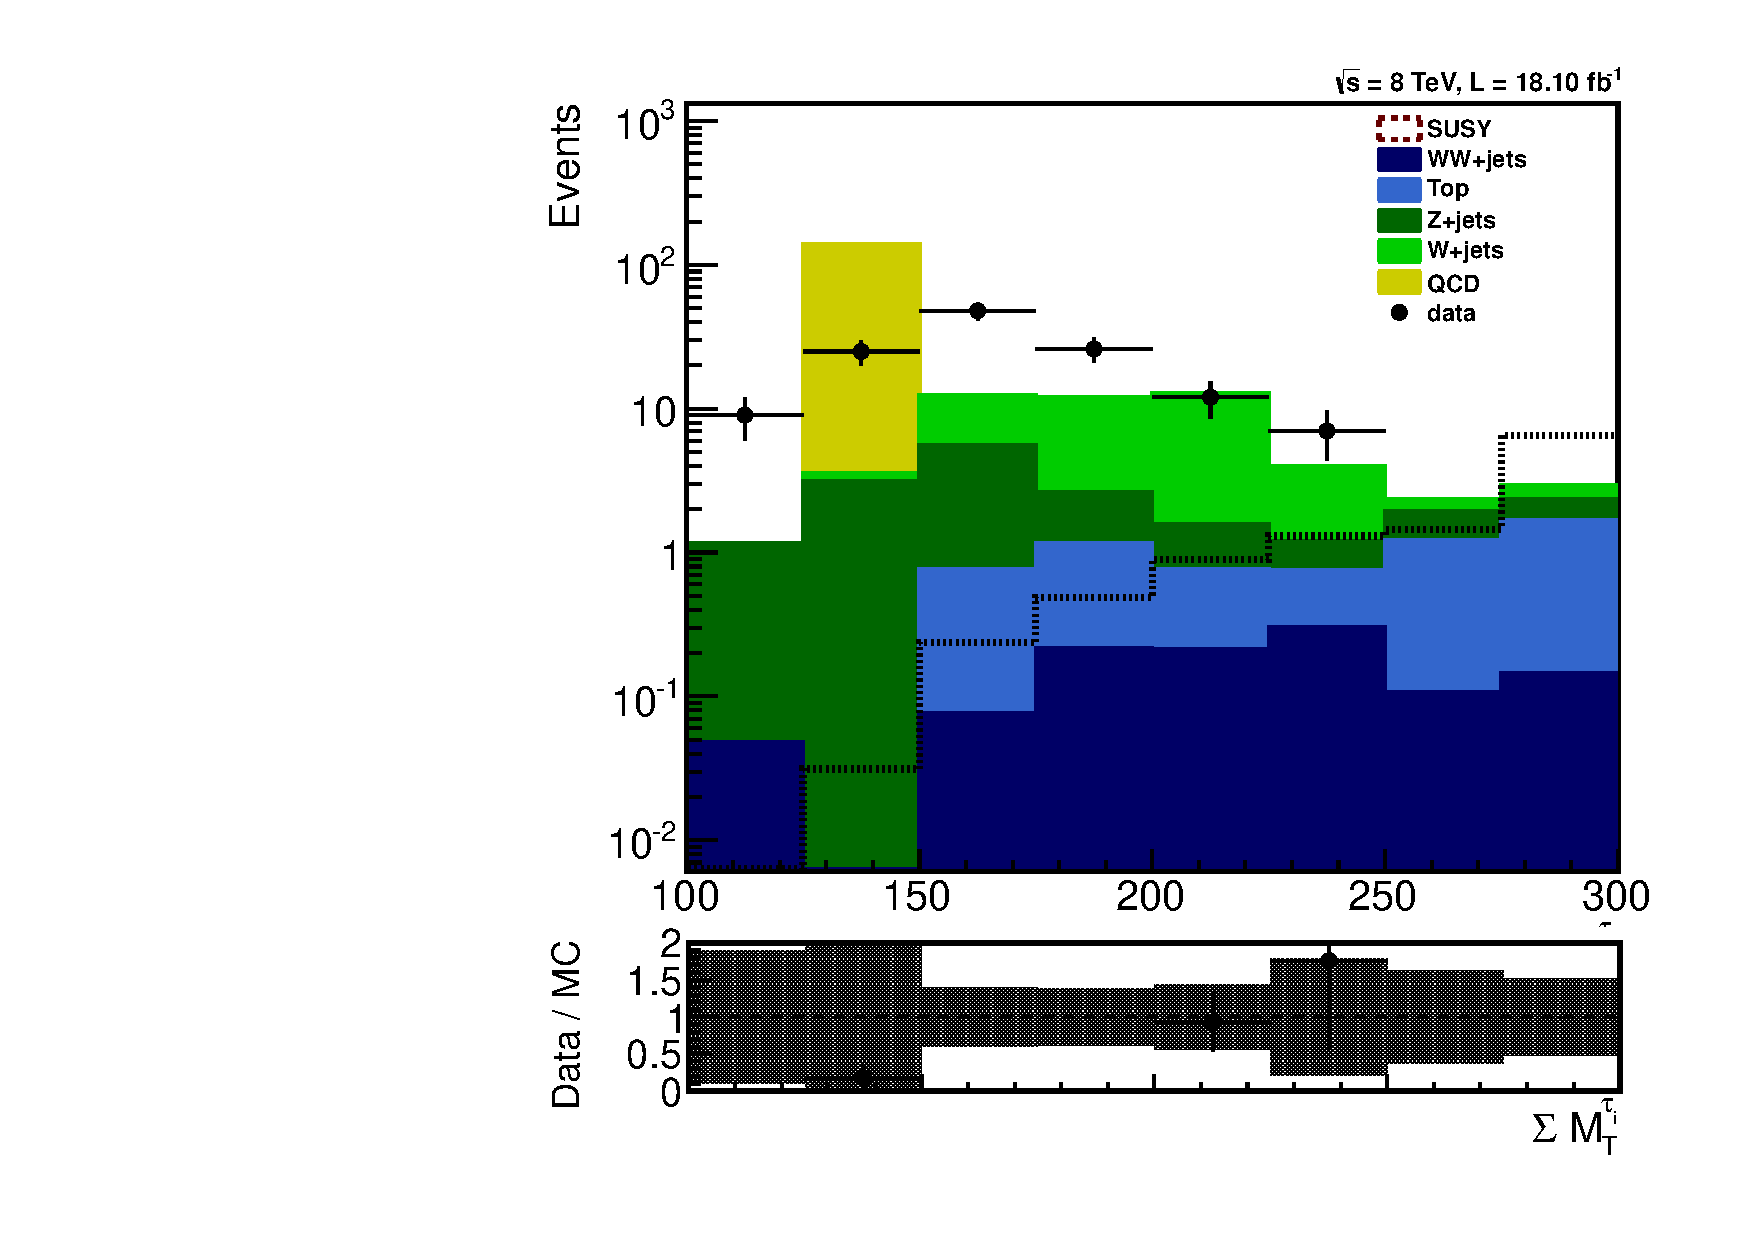
\includegraphics[angle=0,scale=0.35]{TauTauFigs/SumMT_8bins.pdf} \\
\caption{Left: \mttwo. Right: \SumMT.}
\label{fig:comparison}
\end{figure}

\subsection{\texorpdfstring{$\leptonTau$ Channel}{lepton-tau Channel}}
\label{sect:leptonTauCuts}
In lepton ($e$ and $\mu$) $+$ \Tau channels, tight isolated $\Tau$ objects are selected. To reduce the rate of the fake $\Tau$'s orginated from $e$ and $\mu$, the same cuts on the discriminators against $e$ and $\mu$ which are used in the Higgs search analysis \cite{CMS_AN_2013-188} have been applied. In $e + \Tau$ channel, $\Tau$ objects which pass \emph{MediumMVA3Rejection} against $e$ and the \emph{LooseMuon2RejectionPF} discriminator against $\mu$ are selected. In the $\mu + \Tau$ channel, the tight working point of the \emph{Muon2Rejection} is requested and the Loose working point of the discriminator against electron is applied.

$\mu$'s with $\PT > 20 \GeVc$ and $|\eta|<2.1$ are selected in the $\mu + \Tau$ channel. The $\mu$'s should pass tight particle flow identification and a tight cut ($<0.1$) on the isolation.
 
In $e + \Tau$ channel, each event is requested to have an electron with $\PT >25 \GeVc$ in the $|\eta| < 2.1 $ region. A tight cut of $0.1$ on the isolation and $0.1$ on the $dZ$ of the selected electron are also applied.

To suppress dilepton and multilepton backgrounds, events with an extra $e$ or $\mu$ with $\PT >10 \GeV$ are rejected. For the extra electron, a wider window of $|\eta|<2.3$ is scanned and a looser isolation cut of $0.2$ is applied. To veto the extra $\mu$, a selection similar to the $\mu$ selection in $\mu+\tau$ channel is applied.

After requesting two opposite sign leptons in the events, a loose cut on MET $(30 \GeV)$ is applied to suppress QCD events. As there is no b-quark in the signal, rejecting events with one or more b-tagged jets with $\PT > 20 \GeV$ helps a lot in reducing $t\bar{t}$ and $W+b$ backgrounds.

To reject QCD low mass resonances, the invariant mass of the lepton and the $\Tau$ is requested to be greater than $15\ \GeV$. Another cut on the invariant mass of the di-lepton system is applied to remove the peak of the $Z+jets$ events. It has been found that the visible mass of the $Z\to\tau\tau\to\,e +\Tau$ moves to $60 \pm 15 GeV$ due to mis-reconstruction of the energy of the $\Tau$ and also the missing energy due to the decay of the $\tau$ to electron. So the events with invariant mass in the range of $[45,75]$ are cutted away. The minimum angle in the transverse plane between the \MET and the jets with \PT $>$ 40 \GeVc and $|\eta| <$ 5.0 is asked to be greater than 1.0. As the last pre-selection cut, events with $MT2<40 GeV$ are discarded to kill the bulk of the QCD events and get rid of related uncertainities due to mis-reconstruction of the QCD events. As it has mentioned above, the signal events are expected to have high $MT2$ values and are not removed with such a cut.

\begin{table}
\begin{center}
\begin{tiny}
\begin{tabular}{lrrrrrrlr}
\hline
\hline
 & SUSY(380,1) & QCD & VV & Wtolnu & DY & Top & Total Bkg & Data\\
\hline
\hline
\MET,b,DiLepton Selection & 20.49 & 6748.66 & 589.41 & 46139.56 & 17071.56 & 1845.78 & 72394.97$\pm$2147.82 & 76066\\
Extra Lepton Veto & 20.49 & 6477.95 & 582.79 & 46120.60 & 17039.83 & 1820.77 & 72041.94$\pm$2130.68 & 75992\\
Cuts on $m_{\mu\Tau}$ & 19.89 & 6072.89 & 574.26 & 45438.09 & 15867.28 & 1794.82 & 69747.33$\pm$2121.47 & 73459\\
$\mindphifour > 1.0$ & 12.70 & 2271.96 & 198.61 & 11416.01 & 3169.72 & 693.16 & 17749.46$\pm$1498.73 & 19761\\
$\mttwo > 40 \GeV$ & 9.86 & 1514.64 & 82.14 & 4466.30 & 68.90 & 251.07 & 6383.05$\pm$1478.31 & 5446\\
\hline
$\mttwo > 90 \GeV$ & 5.69 & 0.00 & 1.57 & 16.1 & 1.82 & 0.64 & 20.21$\pm$4.24 & 25\\
$\tauMT > 200 \GeV$ & 3.47 & 0.00 & 0.05 & 1.2 & 0.38 & 0.02 & 1.74$\pm$0.63 & 3\\
\hline
\hline
\end{tabular}
\caption{Cut-flow-table for $e-\Tau$ channel}
\label{tbl:cutflowtableeletau}
\end{tiny}
\end{center}
\end{table}

\begin{table}
\begin{center}
\begin{tiny}
\begin{tabular}{lrrrrrrlr}
\hline
\hline
 & SUSY(380,1) & QCD & VV & Wtolnu & DY & Top & Total Bkg & Data\\
\hline
\hline
\MET, b, DiLeptons & 18.28 & 6791.27 & 1778.41 & 79084.31 & 37000.63 & 4433.53 & 129088.14$\pm$3009.89 & 121644\\
Extra Lepton Veto & 16.33 & 5192.66 & 1034.93 & 77139.4 & 32166.18 & 2972.25 & 118505.41$\pm$2601.51 & 111344\\
Cuts on $m_{\mu\Tau}$ & 13.68 & 1721.45 & 759.7 & 46551.75 & 6963.01 & 2128.4 & 58124.31$\pm$1262.89 & 55282\\
$\mindphifour > 1.0$ & 11.29 & 70.87 & 382.9 & 19592.59 & 4130.47 & 1129.26 & 25306.09$\pm$214.76 & 26955\\
$\mttwo > 40\GeV$ & 8.18 & 0 & 164.59 & 8558.78 & 157.33 & 427.51 & 9308.22$\pm$132.94 & 9253\\
\hline
$\mttwo > 90\GeV$ & 3.5 & 0 & 2.19 & 17.67 & 1.17 & 1.15 & 22.18$\pm$5.20 & 30\\
$\tauMT > 200\GeV$ & 2.41 & 0 & 0.34 & 0.79 & 0.28 & 0 & 1.40$\pm$0.49 & 5\\
\hline
\hline
\end{tabular}
\caption{Cut-flow-table for $\mu-\Tau$ channel}
\label{tbl:cutflowtablemuotau}
\end{tiny}
\end{center}
\end{table}

The cut flow tables for the $e$/$\mu$ $\,+\tau$ pre-selections are shown in tables~\ref{tbl:cutflowtableeletau} and~\ref{tbl:cutflowtablemuotau} respectively. The distribution of the \PT of the $\Tau$ and $MET$ in the pre-selected events in both channels are shown in FIGS~\ref{fig:datamceletau} and~\ref{fig:datamcmuotau} . The good agreement between data and MC confirms that the needed correction factors are considrred carefully.

\begin{figure}[htbp]
\centering
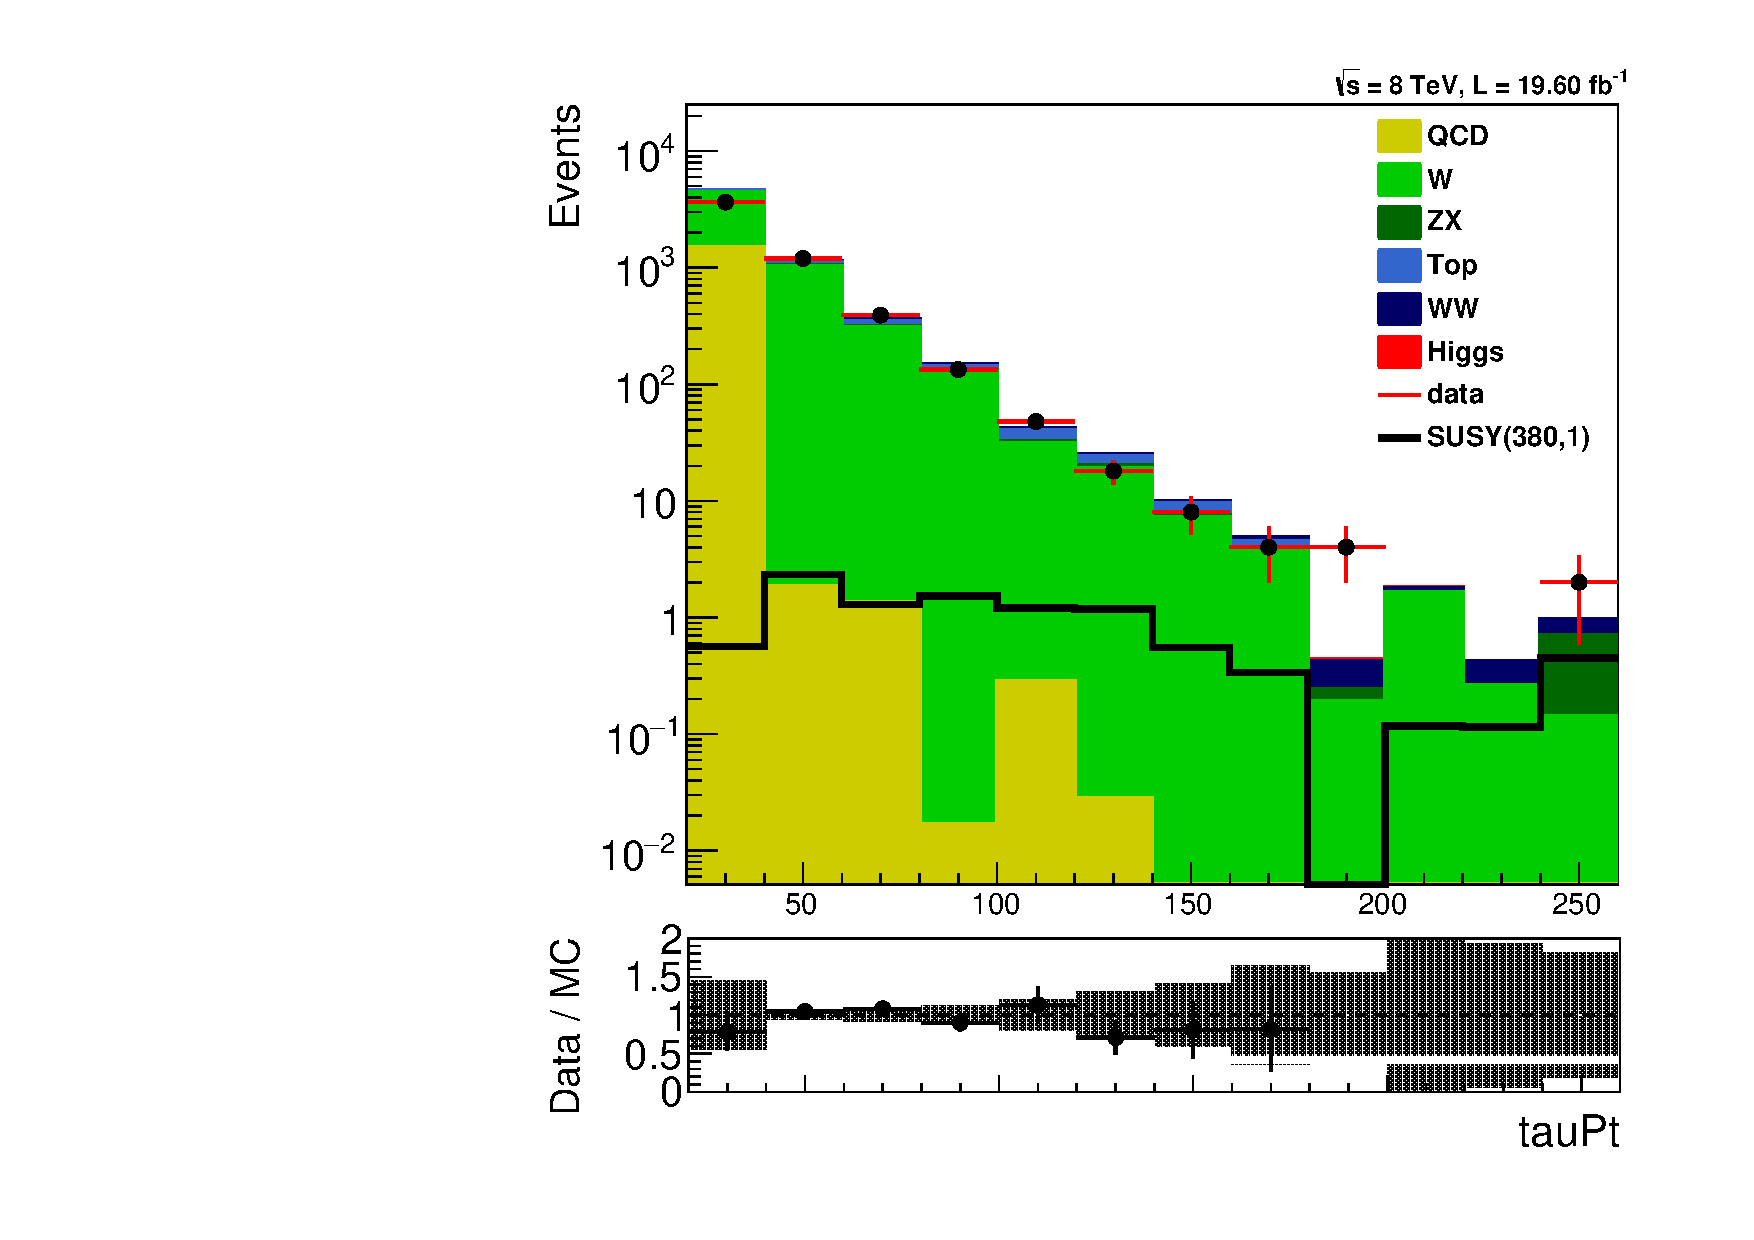
\includegraphics[angle=0,scale=0.35]{SelectionEleTau/TauPt.pdf}
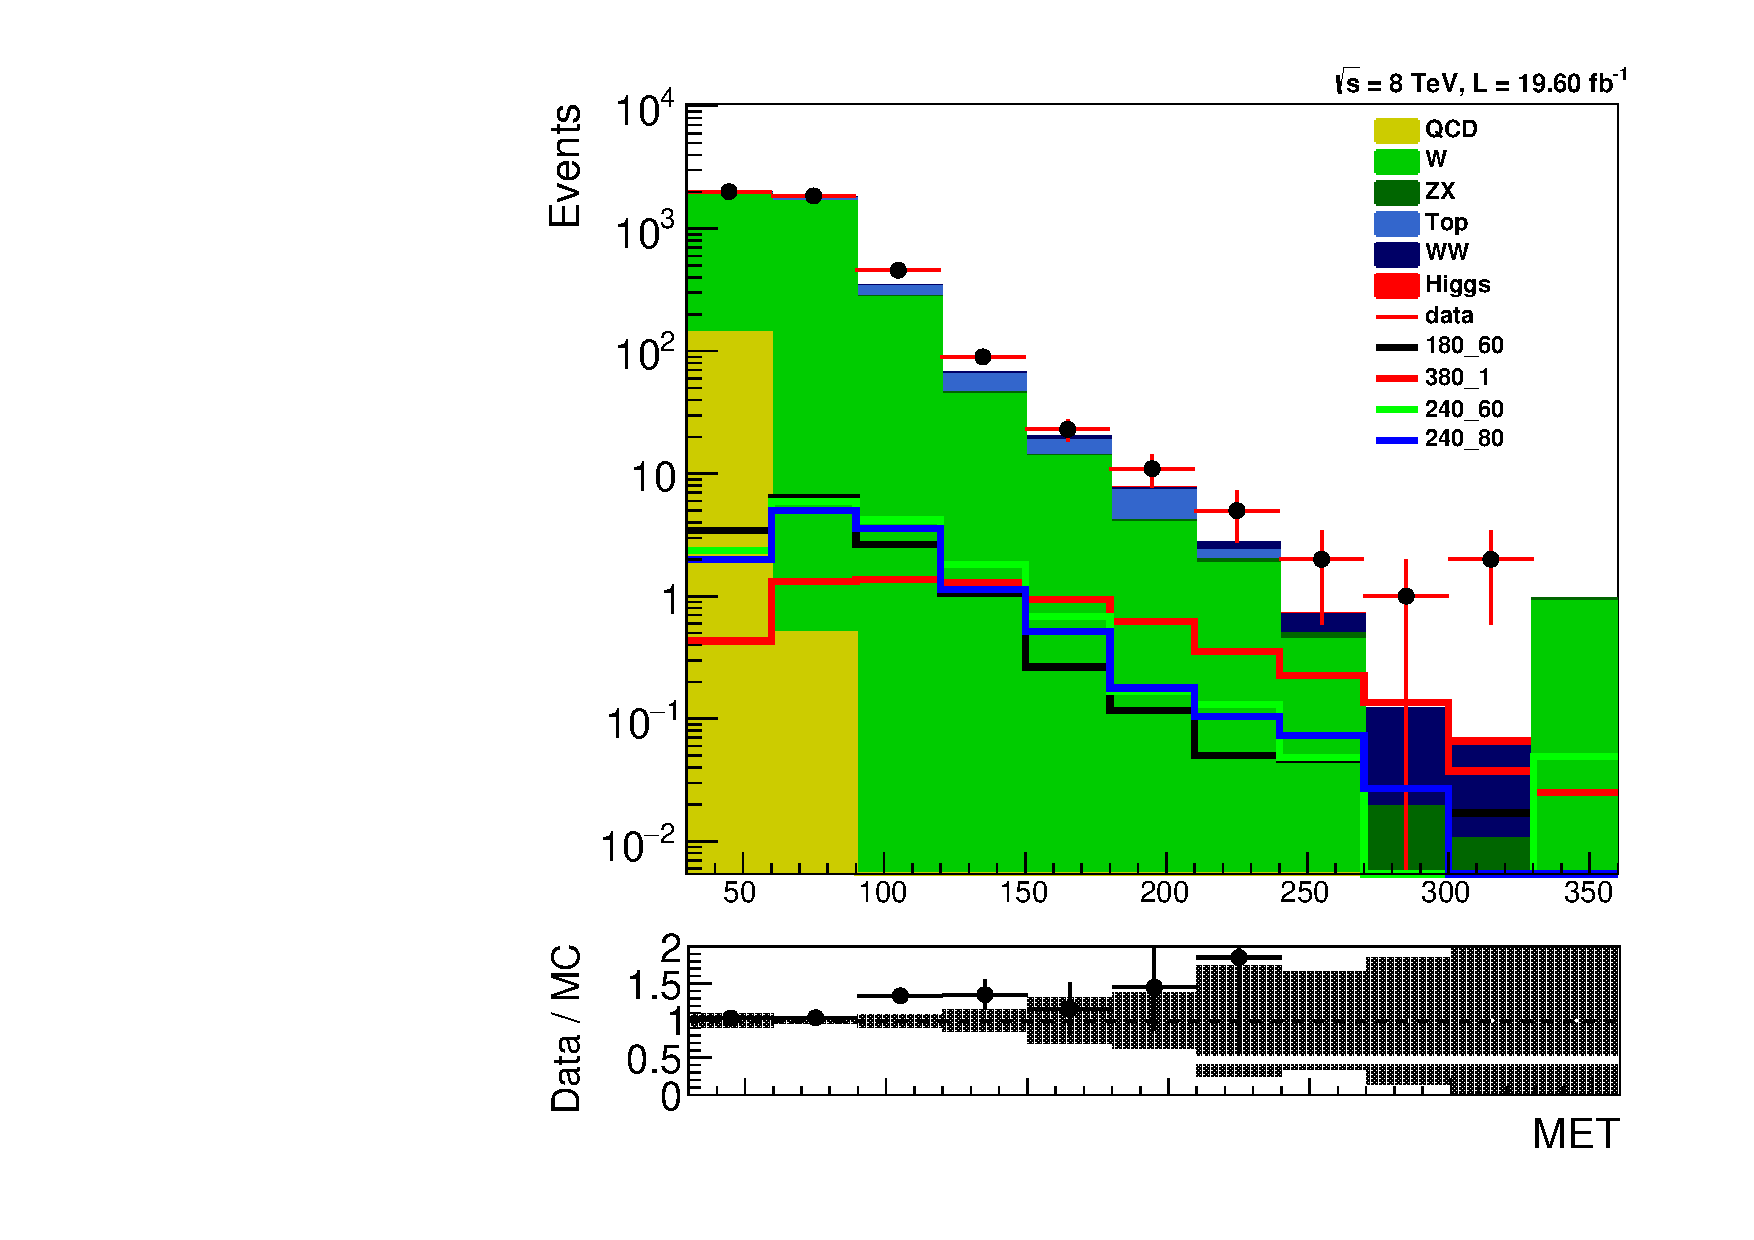
\includegraphics[angle=0,scale=0.35]{SelectionEleTau/MET.pdf}
\caption{Left: \Tau\PT. Right: \MET. in Preselected $e-\Tau$ events.}
\label{fig:datamceletau}
\end{figure}

\begin{figure}[htbp]
\centering
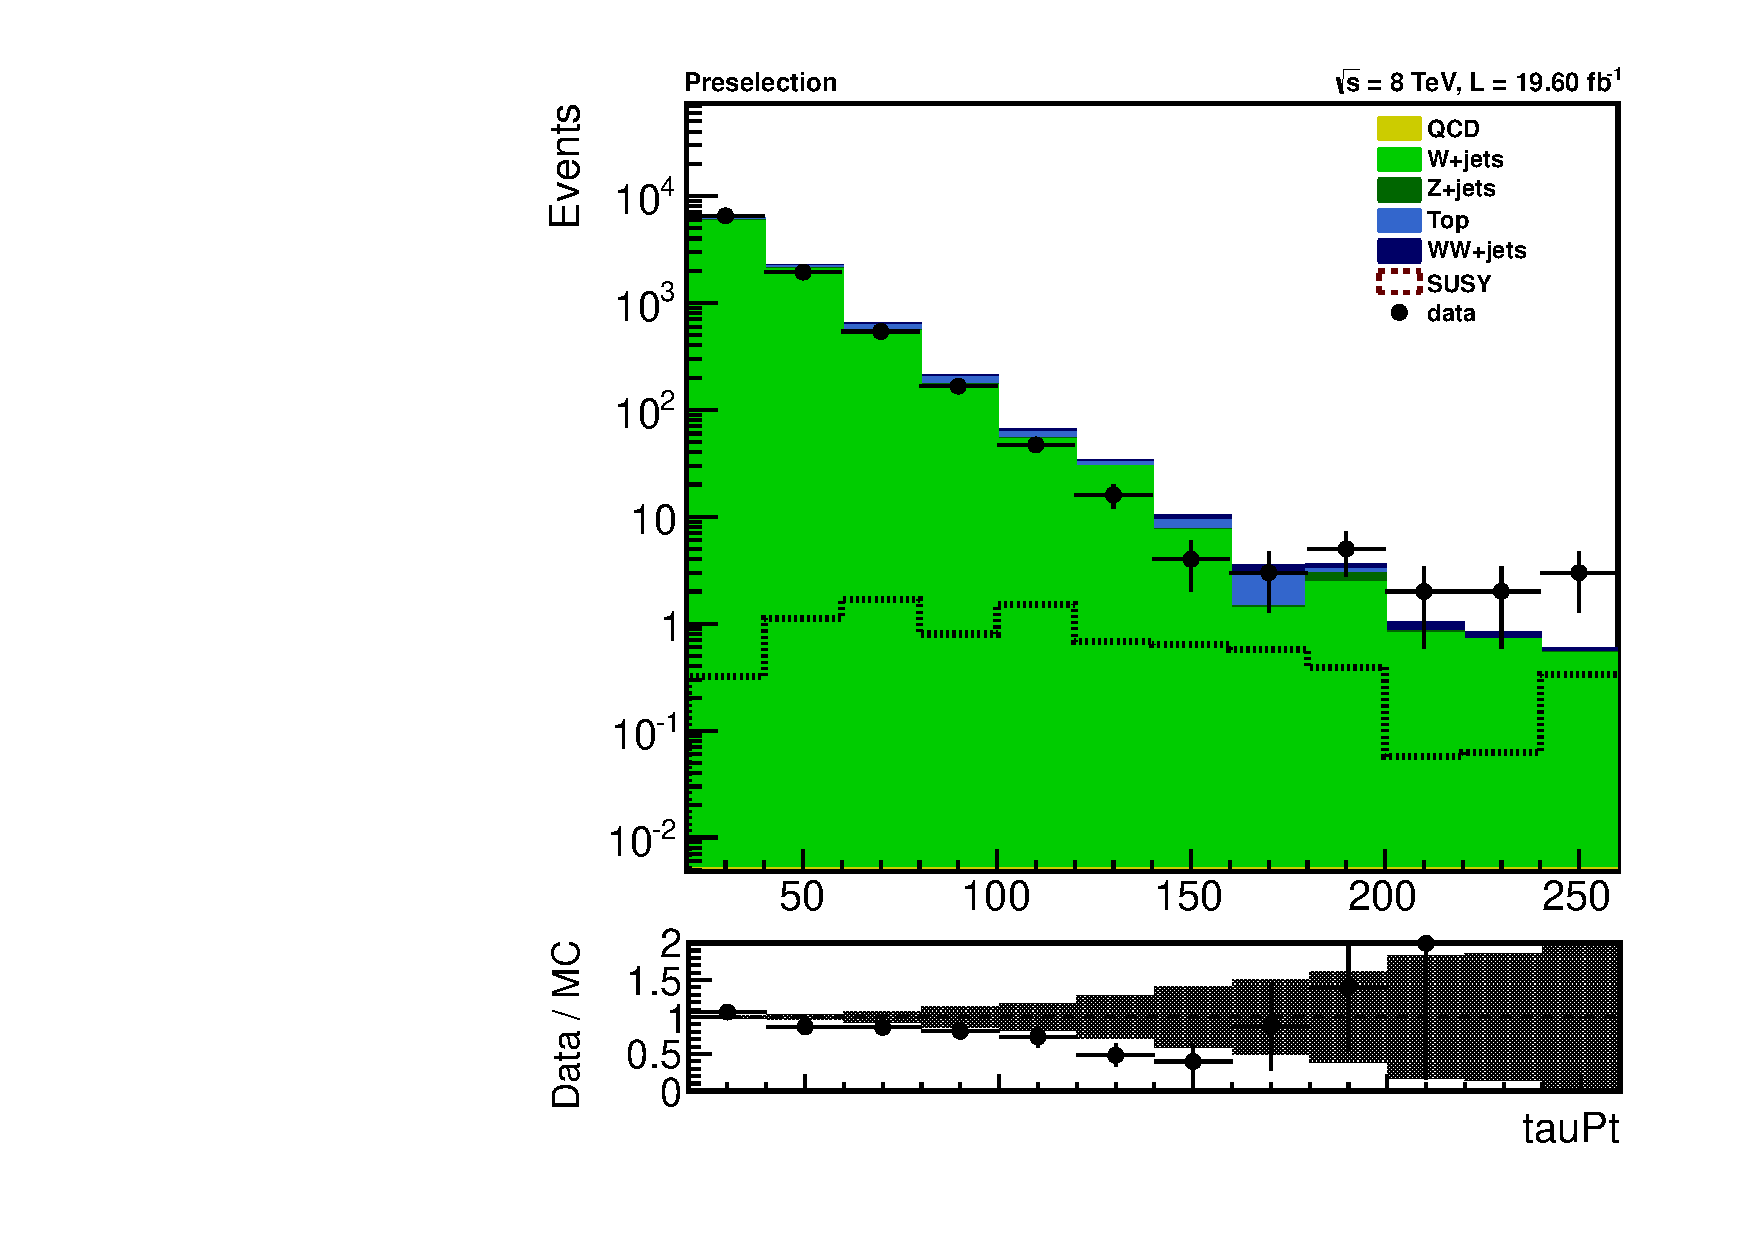
\includegraphics[angle=0,scale=0.35]{SelectionMuTau/tauPt_muTau.pdf}
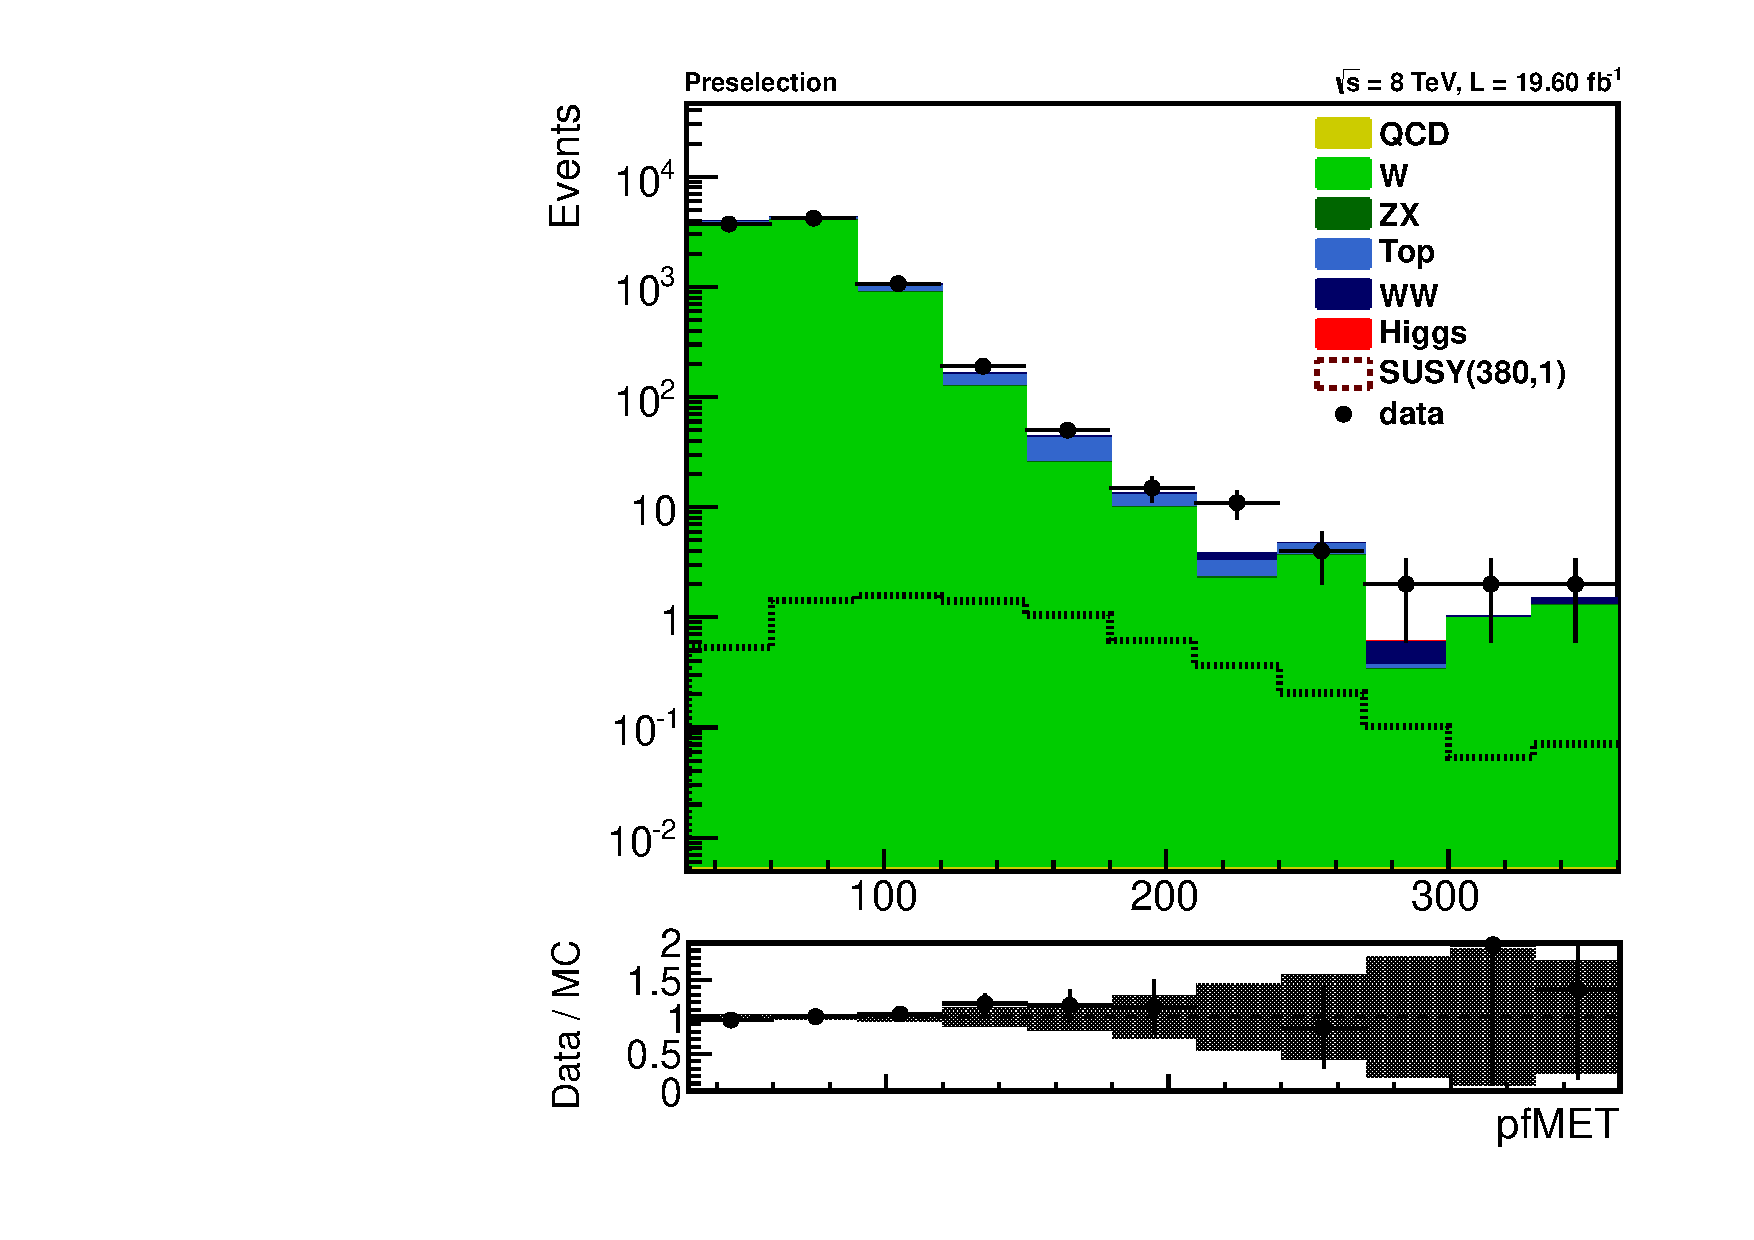
\includegraphics[angle=0,scale=0.35]{SelectionMuTau/pfMET_muTau.pdf}
\caption{Left: \Tau\PT. Right: \MET. in Preselected $\mu-\Tau$ events.}
\label{fig:datamcmuotau}
\end{figure}

Similar to the $\Tau\Tau$ channel, first we find the optimized cut on the $MT2$ to suppress backgrounds especially $W+jet$ events. As it has been shown in FIG~\ref{fig:mt2leptontau}, the best value to cut on, similar to the $\Tau\Tau$ channel is $MT2 > 90 GeV$ for both $e/\mu+\Tau$ channels. Such a high cut on the $MT2$ increases the sensitivity of the study to signal events with high $\chipm$ and $\chiz$ mass differences. We then investigate the shape of different variables for signal and backgrounds and try to find the most optimized cut to have the best exclusion. The most sensitive variable for both channels are found to be the $\Tau$ transverse mass. As it has been shown in FIG~\ref{fig:taumtleptontau}, the best cut value for the high mass difference signal is $M_{T}^{\Tau} > 200 GeV$. You can find the composition of the backgrounds and number of remaining signals for both channels in the last row of the cut flow tables (tables~\ref{tbl:cutflowtableeletau} and~\ref{tbl:cutflowtablemuotau}).

\begin{figure}[htbp]
\centering
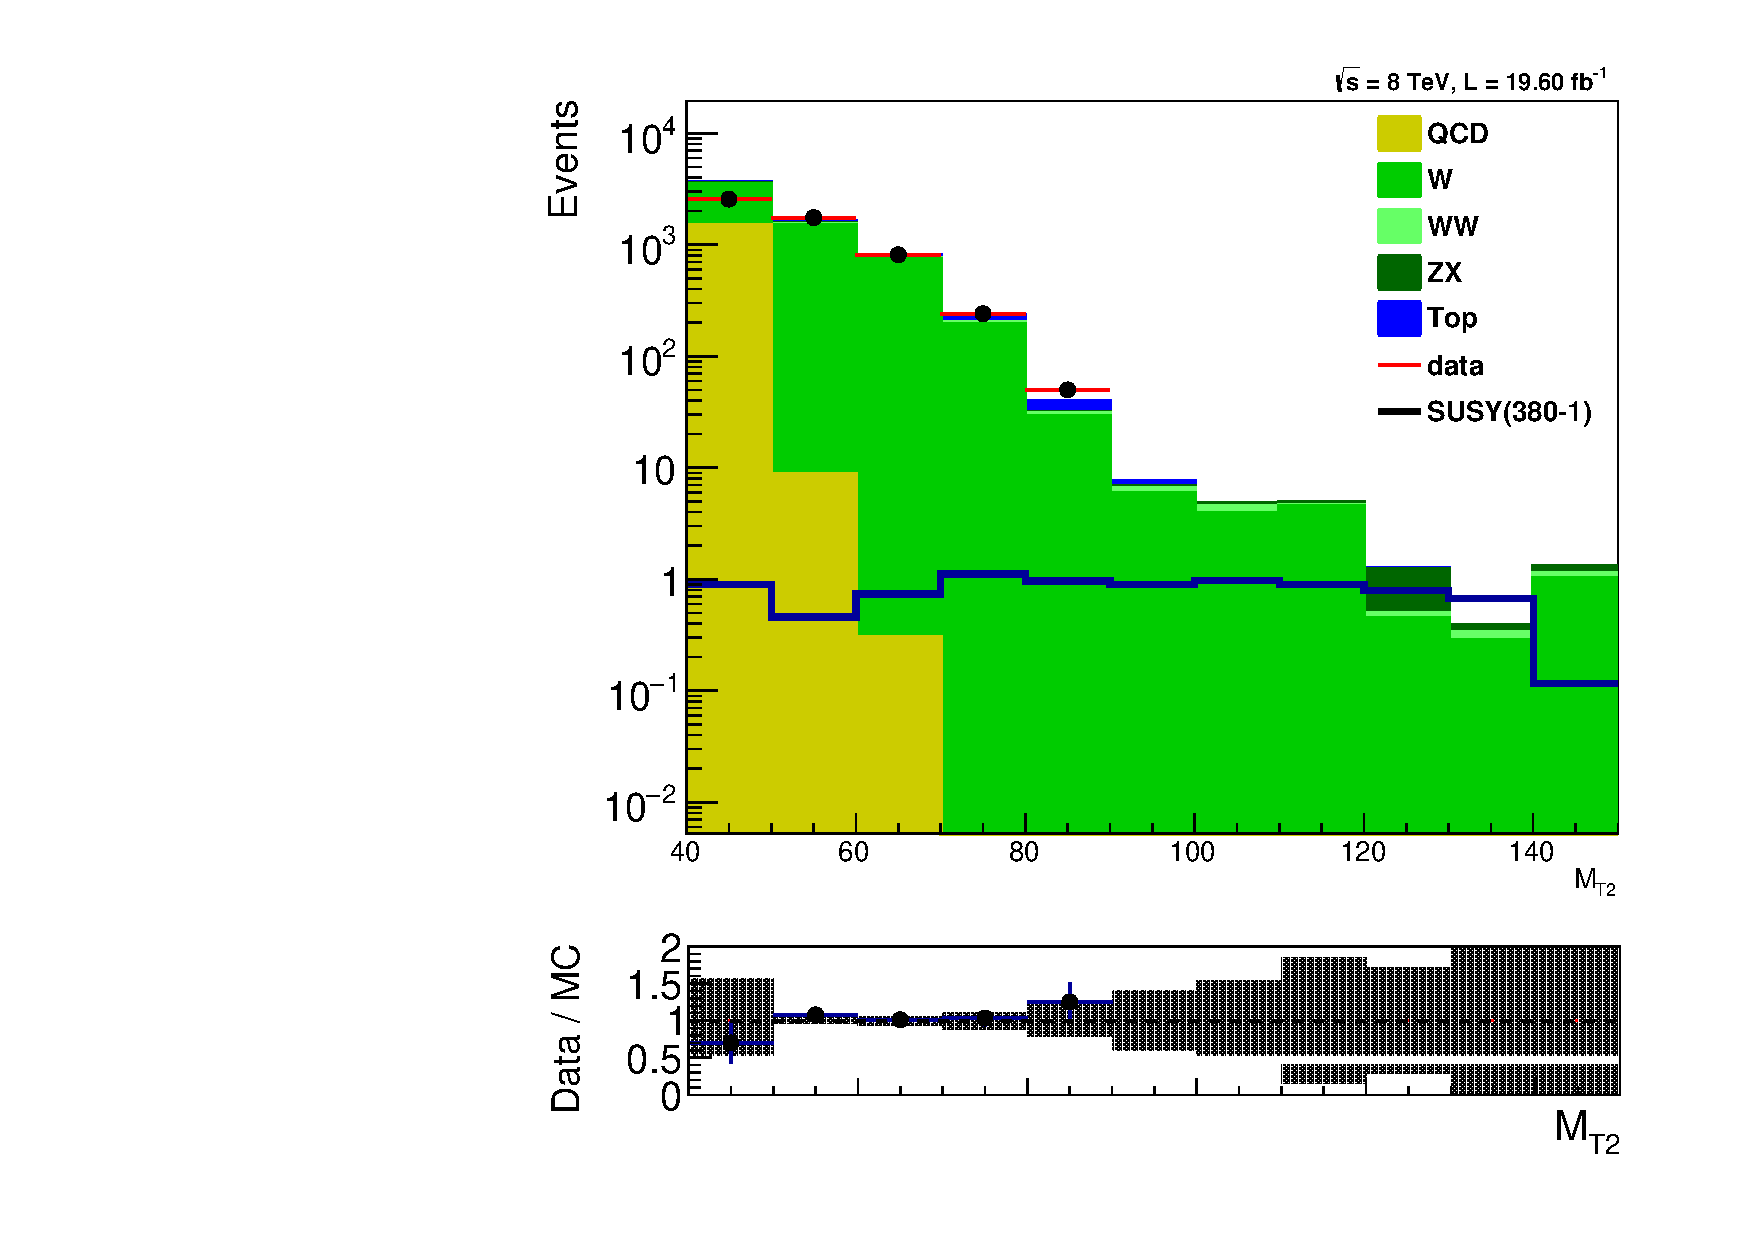
\includegraphics[angle=0,scale=0.35]{SelectionEleTau/MT2.pdf}
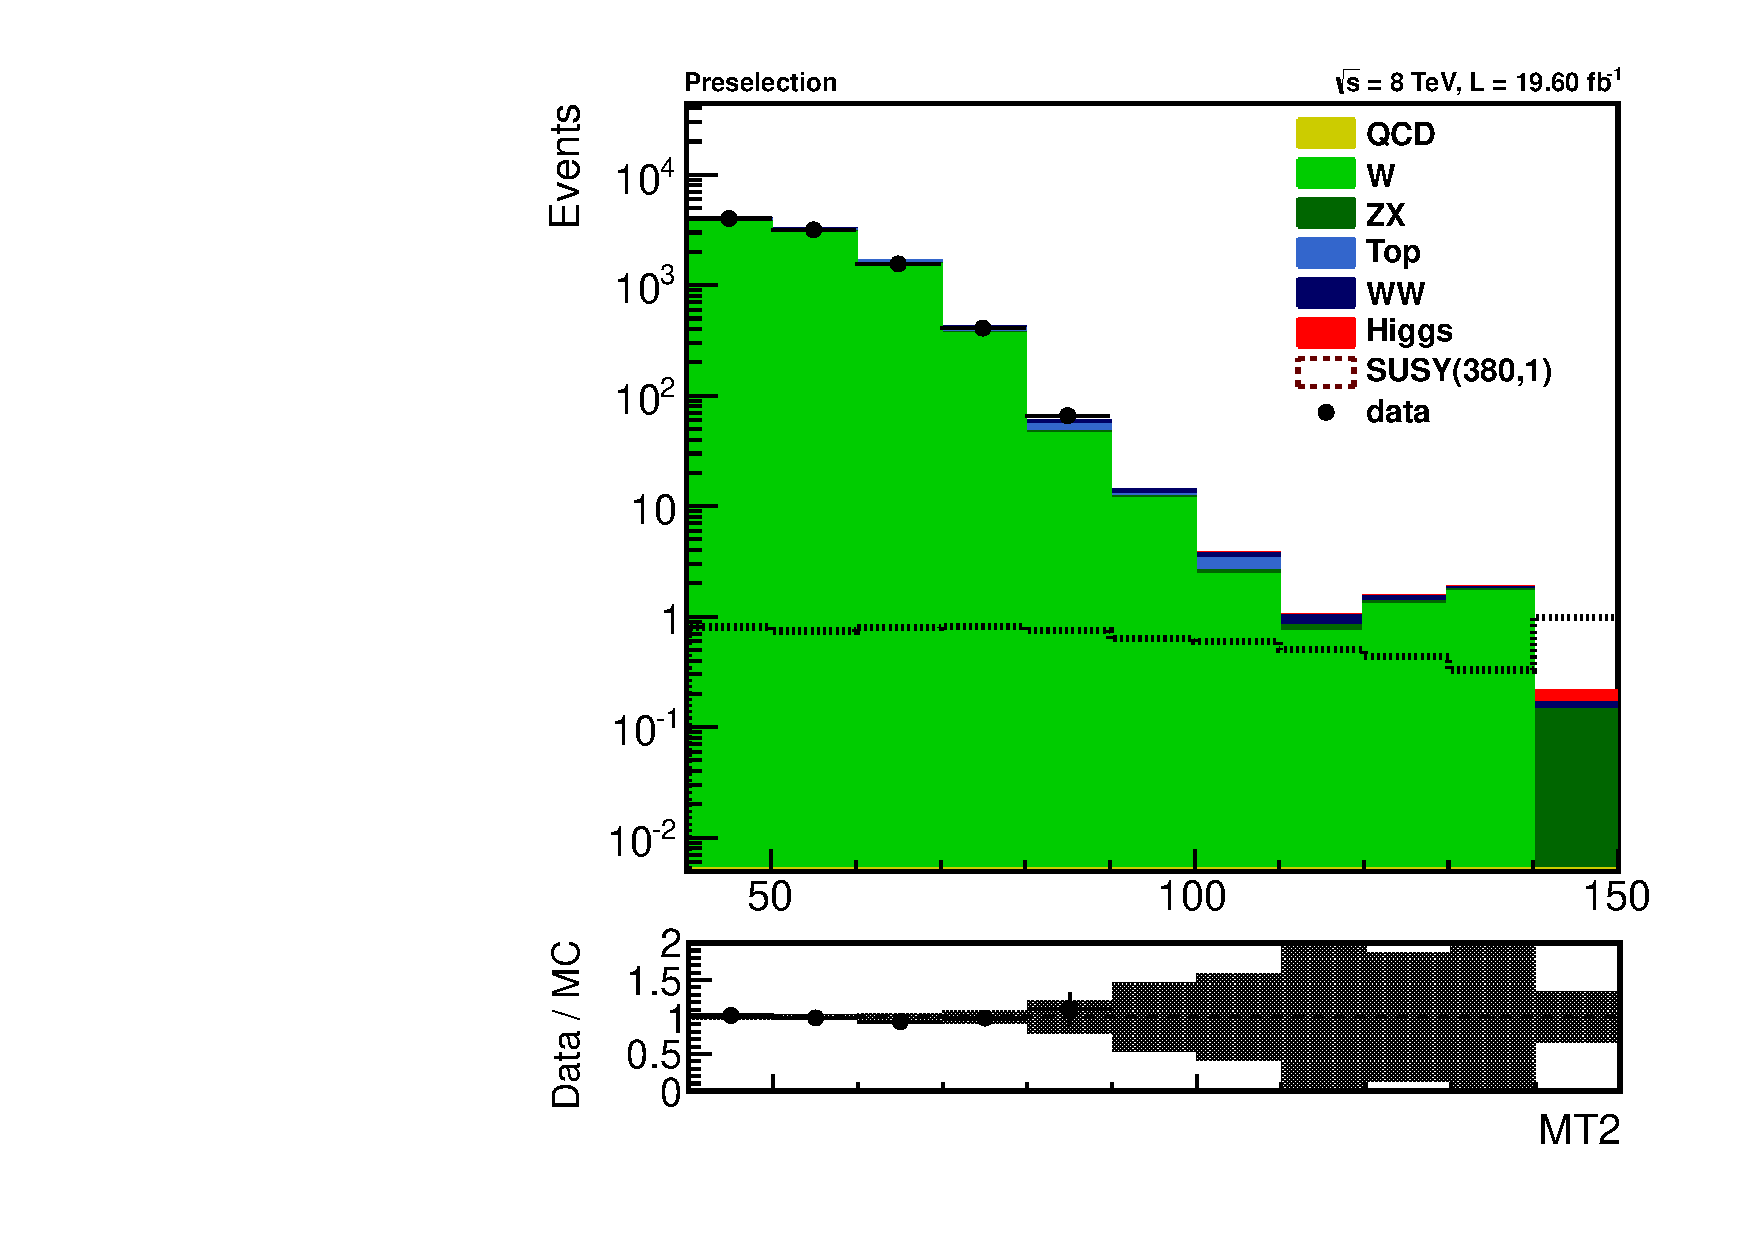
\includegraphics[angle=0,scale=0.35]{SelectionMuTau/MT2_muTau.pdf}
\caption{\mttwo distribution of preselected events in (Left) $e-\Tau$ and (RIGHT) $\mu-\Tau$ channels.}
\label{fig:mt2leptontau}
\end{figure}

\begin{figure}[htbp]
\centering
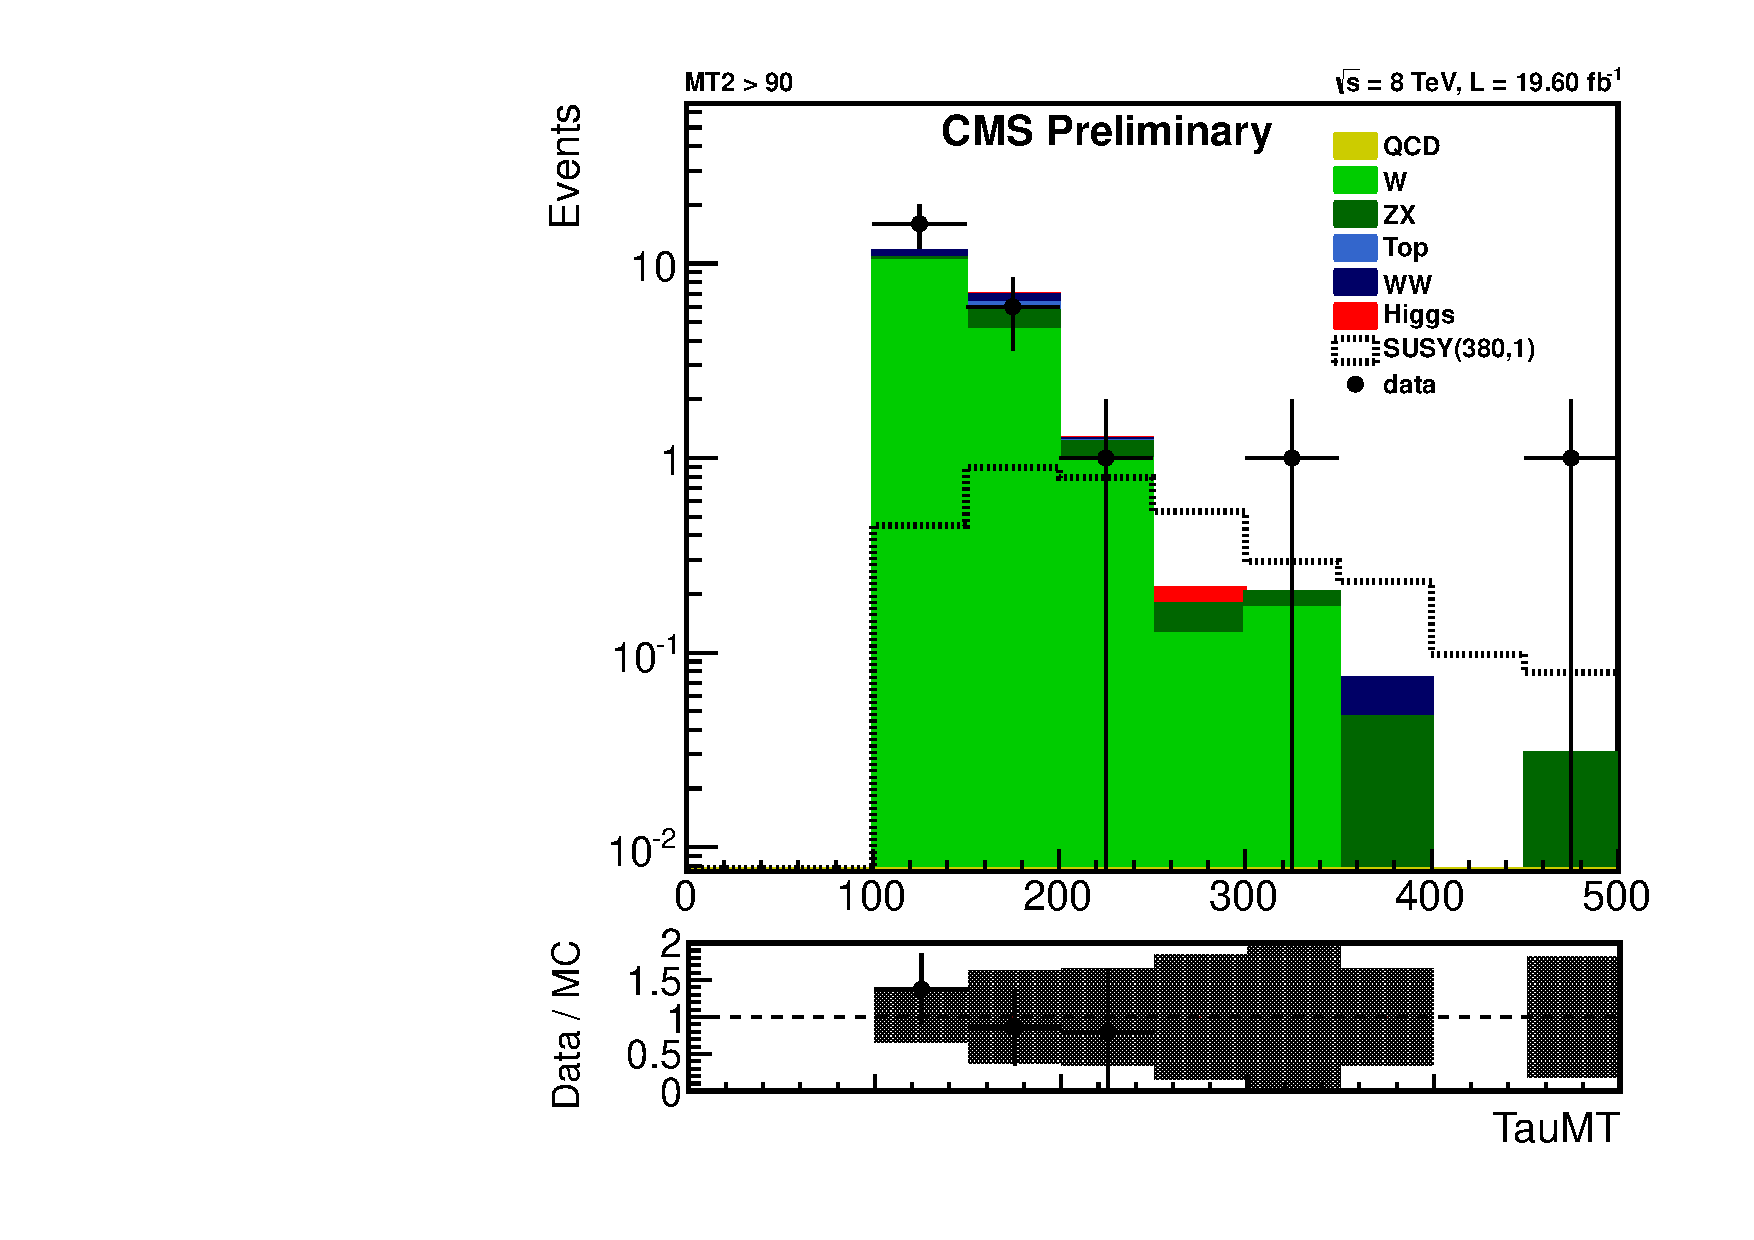
\includegraphics[angle=0,scale=0.35]{SelectionEleTau/TauMT.pdf}
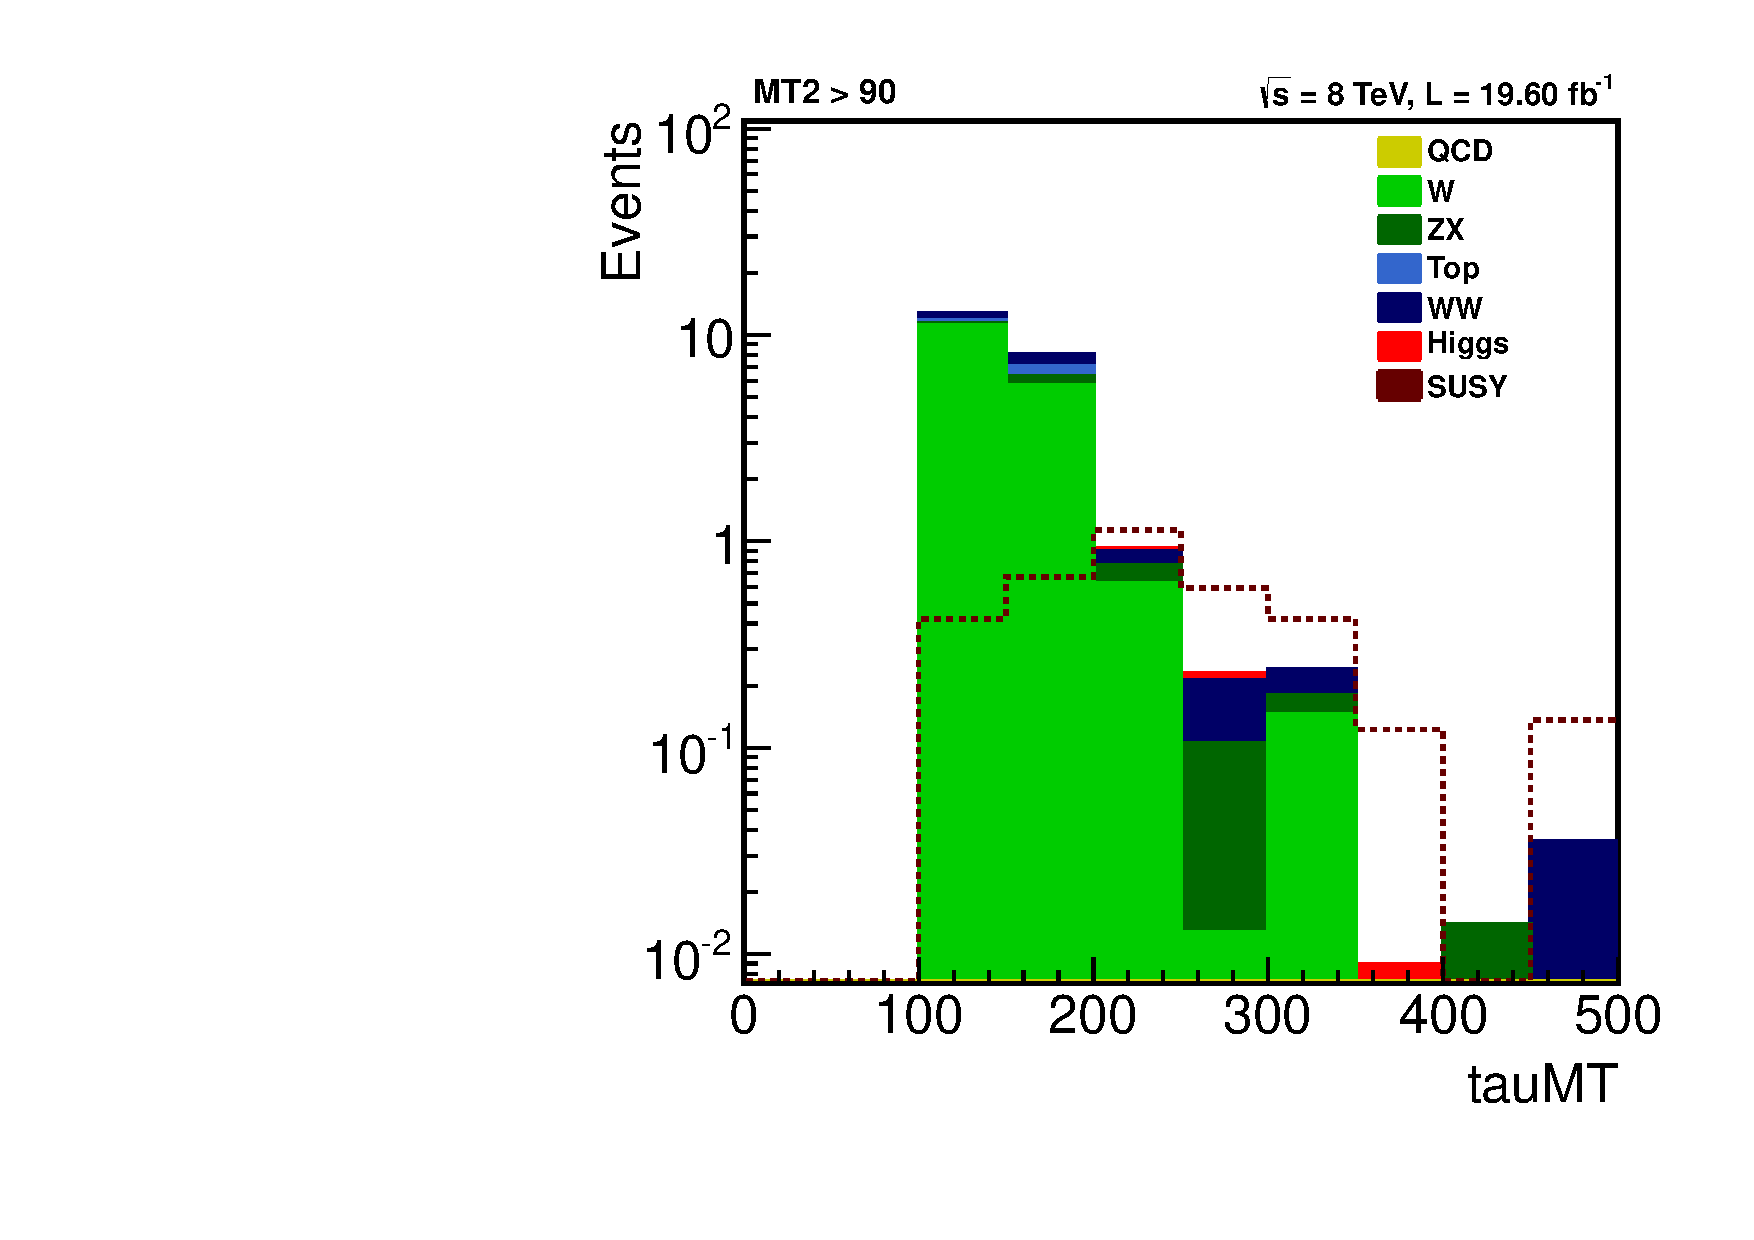
\includegraphics[angle=0,scale=0.35]{SelectionMuTau/tauMT_MuTau.pdf}
\caption{\tauMT distribution for events with $\mttwo>90\GeV$ in (Left) $e-\Tau$ and (RIGHT) $\mu-\Tau$ channels.}
\label{fig:taumtleptontau}
\end{figure}

Opposite to the $\Tau\Tau$ channel, the events with $MT2<90 GeV$ are not useful in electron/$\mu + \tau$ channels because of the contamination of the $W+jets$ events.
